
\numberwithin{definition}{section}
\numberwithin{example}{section}
\numberwithin{equation}{section}
\numberwithin{figure}{section}

\addbibresource{../bib/taiga.bib}
\addbibresource{../bib/tex.bib}
%-----------------------------------------------------------------
\title{Flat predictive models}
\author{\textsc{John Alan McDonald }}
\date{draft of \today}
%-----------------------------------------------------------------
\begin{document}
\maketitle
%-----------------------------------------------------------------

Taiga's implementation of linear models is expressed in a way
that is different from the treatment in most statistics texts.
I happen to think that Taiga's approach is simpler, and better, 
particularly because it allows us to discuss these models as
special cases of a general approach to predictive models.
Whether you agree with that or not, you will need to understand
Taiga's point of view if you want to use it successfullly.

\textit{Flat} means linear or affine.

\section{\label{sec:Linear} Linear spaces and functions}

A \textit{real linear space} 
(commonly refered to as a
\textit{real vector space}) 
\(\mathbb{V}\) is a set of elements, called vectors,
\(\mathsf{v}_0\), \(\mathsf{v}_1\), \ldots that is closed under 
\textit{linear combinations}:
\begin{equation}
\mathsf{v} \; = \; a_0 \mathsf{v}_0 \, + \, a_1 \mathsf{v}_1 
\in \mathbb{V}
\end{equation}
for all \(a_0, a_1 \in \mathbb{R}\).
Note that \(\mathbb{R}\) itself is a linear space under this
definition.

(This can be generalized to other scalar fields,
but \(\mathbb{R}\) is sufficient for this discussion,
and will be assumed in what follows.)

A \textit{linear function} \(\mathsf{f}\) from linear space
\(\mathbb{V}\) to linear space \(\mathbb{W}\) 
preserves linear combinations:
\begin{equation}
\mathsf{f}(a_0 \mathsf{v}_0 + a_1 \mathsf{v}_1 ) 
\; = \;
a_0 \mathsf{f}(\mathsf{v}_0) \, + \, 
a_1 \mathsf{f}(\mathsf{v}_1)
\end{equation}
A \textit{linear functional} is just a real-valued linear
function: \(\mathsf{f} : \mathbb{V} \rightarrow \mathbb{R}\).

The canonical linear space is \(\mathbb{R}^n\),
which we will take here to be the set of tuples of \(n\) real
numbers. Implementations in Clojure/Java will most often
approximate real tuples with instances of \texttt{double[n]},
often with instances of classes wrapping \texttt{double[n]},
and occasionally with \texttt{List<Number>.} 

Note that the set of linear functions between two linear
spaces, \(\mathcal{L}(\mathbb{V},\mathbb{W})\) is itself a linear
space. 

In fact, given any set of functions \(\mathcal{F} = {\mathsf{f} :
\mathbb{D} \rightarrow \mathbb{V}}\), 
from any domain \(\mathbb{D}\) to a 
linear space \(\mathbb{V}\),
we get a linear space by closing those functions under linear
combinations of their values:
\(\mathbb{F} = \{ \mathsf{f}() = \sum_i a_i\mathsf{f_i}() \; : \;
\mathsf{f_i} \in \mathcal{F}, a_i \in \mathbb{R} \}\)

See Halmos \cite{halmos-1958} for thorough background.

\section{Inner product space}

An \textit{inner product space} is a linear space
together with an \textit{inner product}, a symmetric,
positive semidefinite, bilinear function of 2 arguments:
\begin{equation}
\begin{split}
\mathrm{dot}(\mathsf{v_0},\mathsf{v_1}) & =
\mathrm{dot}(\mathsf{v_1},\mathsf{v_0}) \\
\mathrm{dot}(\mathsf{v},\mathsf{v}) & \geq 0 \\
\mathrm{dot}(\mathsf{v},a_0\mathsf{v_0}+a_1\mathsf{v_1}) & =
a_0\mathrm{dot}(\mathsf{v},\mathsf{v_0}) + 
a_1\mathrm{dot}(\mathsf{v},\mathsf{v_1})
\end{split} 
\end{equation}

Skipping some details, we can identify
the linear functionals on an inner product space with the 
vectors in that space:
\begin{equation}
\mathsf{v}^{\dagger}(\mathsf{w}) =
\mathrm{dot}(\mathsf{v},\mathsf{w}) \forall \mathsf{w} \in
\mathbb{V}
\end{equation}

L2 norm is
\(\|\mathsf{v}\|_2 = \sqrt(\mathrm{dot}(\mathsf{v},\mathsf{v})
\) 

L2 distance is \(\|\mathsf{v_0}-\mathsf{v_0}\|_2 \). 

\section{\label{sec:Affine} Affine spaces and functions}

An \textit{affine space} is similar to a linear space, only
closed under \textit{affine combinations} rather than linear.
That is,
\(\mathbb{A}\) is a set of elements, called points,
\(\mathsf{p}_0\), \(\mathsf{p}_1\), \ldots such that:
\begin{equation}
\mathsf{p} \; = \; a_0 \mathsf{p}_0 \, + \, a_1 \mathsf{p}_1 
\in \mathbb{A} \forall \mathsf{p}_0, \mathsf{p}_1 \in
\mathbb{A}; a_0, a_1 \in \mathbb{R}; a_0 + a_1 = 1
\end{equation}
for all \(a_0, a_1 \in \mathbb{R}\).
The key distinction is the constraint that \(a_0 + a_1 = 1\).

Abstract differences\(\rightarrow\) linear translation space.

Note that every linear space is automatically an affine space,
but not the reverse.

A canonical example of an affine space that is not a linear
space is a hyperplane in \(\mathbb{R}^n\) that doesn't go thru
the origin, such as the set of all vectors whose first
coordinate is 1. (TODO: picture of such a hyperplance in
\(\mathbb{R}^2\)).

Linearization via equivalence classes of homogeneous
coordinates.

Implementations:
\begin{enumerate}
  \item (Coordinate frame) Pick an origin. Identify elements
  with elements of \( \mathbb{R}^n \). An affine function on 
  \( \mathbb{R}^{m} \mapsto \mathbb{R}^n \) is a linear
  function plus an 'intercept' term in \( \mathbb{R}^n \).
  \item (Linear Lifting) Identity elements with equivalence
  classes in \( \mathbb{R}^{n+1} \). 
  \( [p_0, p_1, \ldots, p_n] \sim [p_0/p_n, p_1/p_n, \ldots, 1]
  \). Every linear function \(\mathbb{R}^{m+1} \mapsto
  \mathbb{R}^{n+1} \) is an affine function on the equivalence classes.
\end{enumerate}

\section{Euclidean space}

 Affine space where translation space is an inner product space.
 
\section{Flat predictive models}

Idea is to restrict model space to linear or affine functions.
Although still probably taught as the default model type,
very tricky to use well. Rigidity leads to lack of
expressiveness and instability, change any training data can
have unbounded effects on predictions far from the change.

\section{Embedding data in flat spaces}

Practical issue is that linear functions only make sense on
linear domains; affine on affine domains (which includes
linear.)

Data comes as lists of records, with attributes some of whose
values are numerical, but many taking value in more complicated
domains (eg an address).

Clojure implementation: record = object; dataset = list of
records; attribute = function.

After numerical attributes, the next simplest are probably
categorical, by which I mean an attribute whose values fall in
some finite set. Tricky issue is whether the set of possible
value is know ahead of time (usually assumed and usually wrong)
or whether every new data set may have new values
(eg USA set of states might change, more common is need to cover
territories missing from a training set, etc.)

Whatever set of attributes we start with, we will need to
construct an embedding of the record objects into a flat space.

\section{Regression}

Codomain is \( \mathbb{R} \), so we want flat functionals.
Complete model is \( \mathsf{g} : \mathbb{D} \rightarrow
\mathbb{R} \) constructed from 
\( \mathsf{e} : \mathbb{D} \rightarrow \mathbb{F}^n \)
and 
\( \mathsf{f} : \mathbb{F}^n \rightarrow \mathbb{R} \) 
via \( \mathsf{g} = \mathsf{f} \circ \mathsf{e} \). 

\section{Training by minimizing L2 cost}

\section{Training by minimizing L1 and quantile cost}

\section{Regularization}

'Ridge regression' = minimize L2 norm of parameter vector;
'Lasso' = L1 norm.
Neither makes sense
\newpage{}
\section{Typesetting}

This document was typeset using Mik\TeX{} $2.9$ \cite{Miktex2017} 
and {\TeX}works $0.6.1$ \cite{Texworks2017} 
on \textsc{Windows} $10$. 
I used \texttt{arara} \cite{arara2017} 
to run \texttt{xelatex}, \texttt{biber}, \texttt{xelatex},  and
\texttt{xelatex}.
An alternative is to call these 4 commands by hand.

I believe only Mik\TeX\  and {\TeX}works are Windows specific; 
the actual typesetting tools should be usable on Linux and MacOS as well.

\begin{figure}[htbp]
\centering
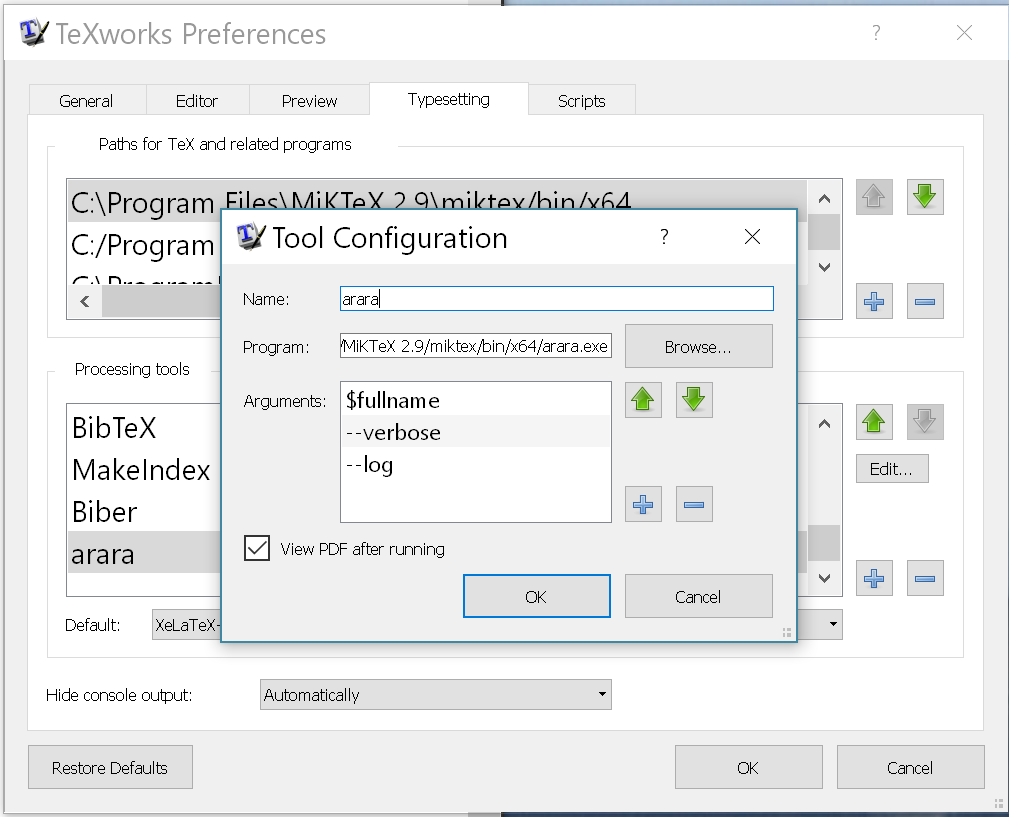
\includegraphics[scale=0.5]{../fig/arara.png}
\caption{Configuring {\TeX}works for \texttt{arara}.}
\label{fig:arara}
\end{figure}

%------------------------------------------------------------------------------
% \begingroup  % Temporarily disable \clearpage to show both lists on one page
%   %\let\clearpage\relax    % http://tex.stackexchange.com/a/14511/104449
%   \renewcommand{\listtheoremname}{List of definitions}
%   \textsf{\listoftheorems[ignoreall, show={definition}]}
% \endgroup
%-------------------------------------------------------------------------------
% \renewcommand{\listfigurename}{Figures}
% \addcontentsline{toc}{chapter}{\listfigurename}
% \begingroup
% \let\onecolumn\twocolumn
% \sffamily
% \listoffigures
% \rmfamily
% \endgroup
%-------------------------------------------------------------------------------
% \renewcommand{\lstlistlistingname}{Code samples}
% \addcontentsline{toc}{chapter}{\lstlistlistingname}
% \begingroup
% \let\onecolumn\twocolumn
% \sffamily
% \lstlistoflistings
% \rmfamily
% \endgroup
%-------------------------------------------------------------------------------
% \renewcommand{\listtheoremname}{Examples}
% \addcontentsline{toc}{chapter}{\lstlistlistingname}
% \begingroup
% \let\onecolumn\twocolumn
% \sffamily
% \listoftheorems
% \rmfamily
% \endgroup
%-------------------------------------------------------------------------------
% \newglossarystyle{mystyle}{%
%  \glossarystyle{altlist}%
%  \renewcommand*{\glossaryentryfield}[5]{%
%    \item[\glsentryitem{##1}\glstarget{##1}{##2}]%
%       :\hspace{1em}##3\glspostdescription\space ##5}%
% }
% \printglossary[title=Glossary,toctitle=Glossary]
%-------------------------------------------------------------------------------
\printbibliography[heading=bibintoc, title={References}]
%-------------------------------------------------------------------------------
% \printindex
%-------------------------------------------------------------------------------

\end{document}
